\clearpage
\subsubsection{STEP 1}
\begin{center}
Insert the Swivel Link into the antenna base and check for tight fit.
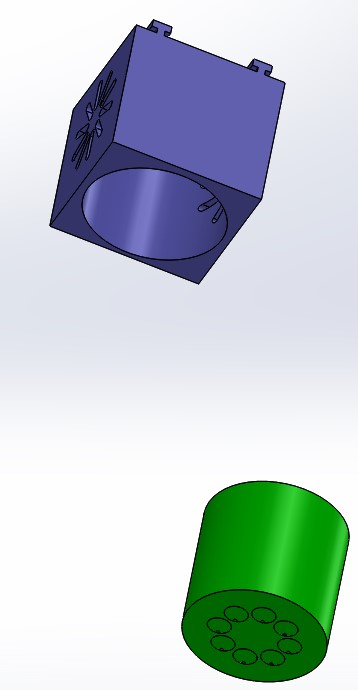
\includegraphics[width=0.85\textwidth]{/a-1-4-ManufacturingWorkingDrawing/b-2-AssemblyInstructionManual/c-Antenna/step1.jpg}
\end{center}
\newline
\subsubsection{STEP 2}
\begin{center}
Align the holes of the antenna support, the crossbar and then swivel link. Insert pin a.
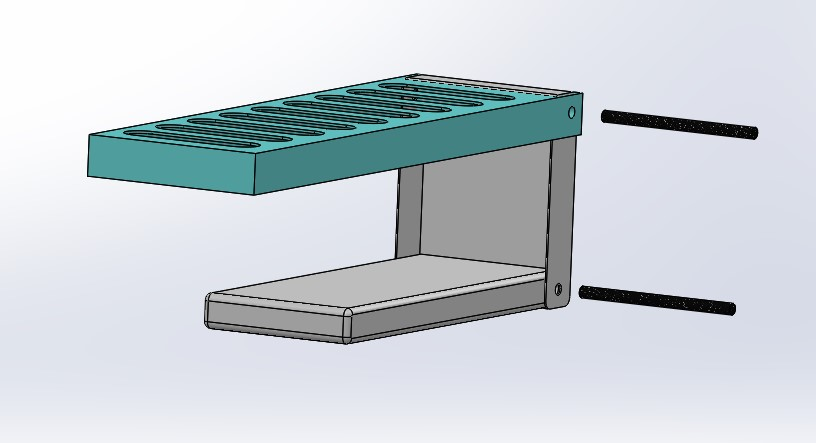
\includegraphics[width=0.85\textwidth]{/a-1-4-ManufacturingWorkingDrawing/b-2-AssemblyInstructionManual/c-Antenna/step2.jpg}
\end{center}
\newline
\subsubsection{STEP 3}
\begin{center}
Align the holes of the crossbar and the signal bar. Insert pin b.
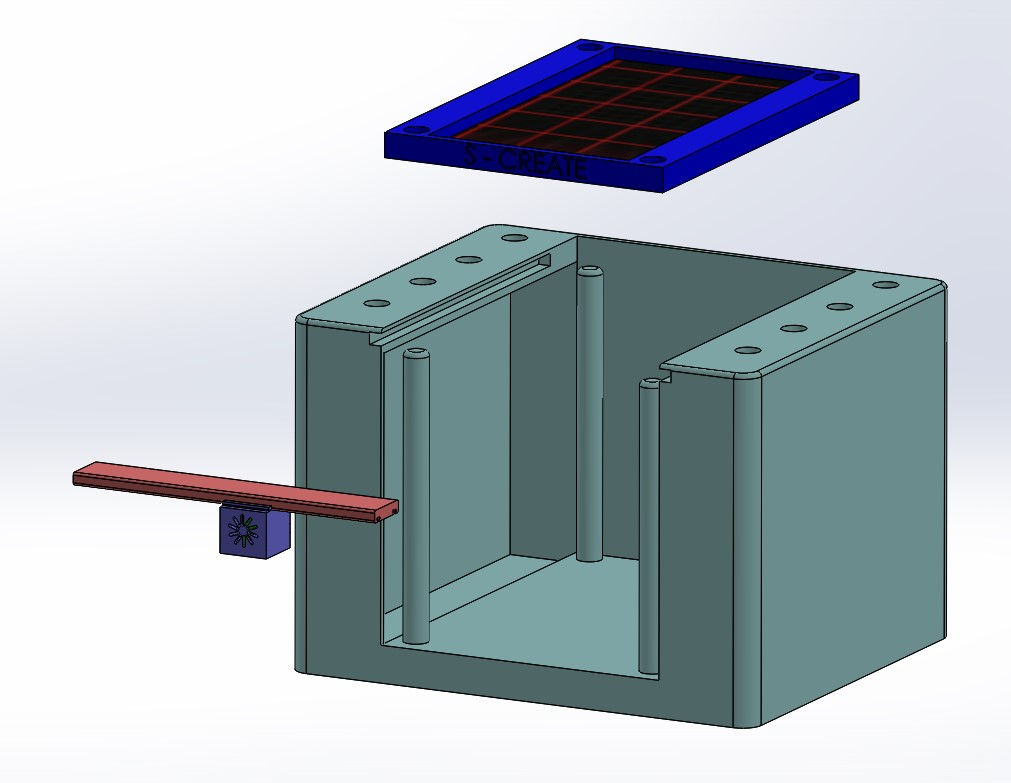
\includegraphics[width=0.85\textwidth]{/a-1-4-ManufacturingWorkingDrawing/b-2-AssemblyInstructionManual/c-Antenna/step3.jpg}
\end{center}
\newline
\subsubsection{STEP 4}
\begin{center}
Align the holes of the signal bar and the retriever. Insert the second pin b.
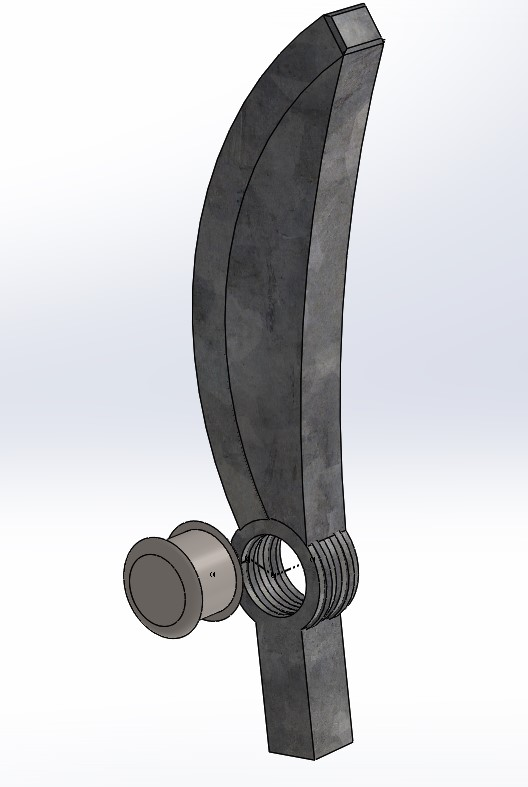
\includegraphics[width=0.85\textwidth]{/a-1-4-ManufacturingWorkingDrawing/b-2-AssemblyInstructionManual/c-Antenna/step4.jpg}
\end{center}
\newline
\subsubsection{STEP 5}
\begin{center}
Attach the ball and socket joint to existing assembly.
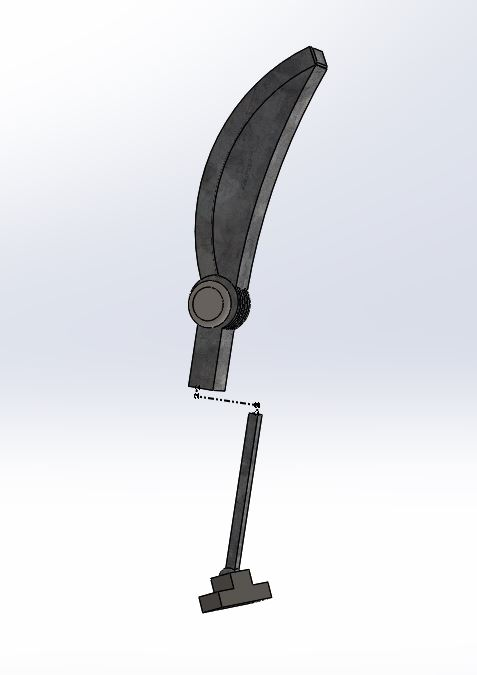
\includegraphics[width=0.85\textwidth]{/a-1-4-ManufacturingWorkingDrawing/b-2-AssemblyInstructionManual/c-Antenna/step5.jpg}
\end{center}
\clearpage
